% Created 2020-04-02 Thu 19:04
% Intended LaTeX compiler: pdflatex
\documentclass[11pt]{article}
\usepackage[utf8]{inputenc}
\usepackage[T1]{fontenc}
\usepackage{graphicx}
\usepackage{grffile}
\usepackage{longtable}
\usepackage{wrapfig}
\usepackage{rotating}
\usepackage[normalem]{ulem}
\usepackage{amsmath}
\usepackage{textcomp}
\usepackage{amssymb}
\usepackage{capt-of}
\usepackage{hyperref}
\usepackage[a4paper, margin=1in]{geometry} \usepackage[utf8]{inputenc}
\usepackage{tikz}
\usetikzlibrary{positioning,arrows}
\setcounter{secnumdepth}{1}
\author{Omar Alkersh - alkersho}
\date{\today}
\title{Assignment 4 Specification and Requirements Documents}
\hypersetup{
 pdfauthor={Omar Alkersh - alkersho},
 pdftitle={Assignment 4 Specification and Requirements Documents},
 pdfkeywords={},
 pdfsubject={},
 pdfcreator={Emacs 26.3 (Org mode 9.3.6)},
 pdflang={English}}
\begin{document}

\maketitle
The specification for \emph{Two Dots} consists of \texttt{Controller}, the main controller in the CV, \texttt{View}, the module responsible for the view, \texttt{BoardT}, the module holding the board information, \texttt{GameState} interface, the interface responsible for the win and lose conditions, and the three implementing modules of \texttt{GameState}.

The game is a 2 dimensional board which consists of coloured dots. The main action of the game is to connect at least two adjacent dots, not diagonally. Connecting dots consumes them, lowering the above dots to fill the gap then populates the empty top spots with new random dots. The win and lose conditions are defined by the game type.

There are three specified game types:

\begin{itemize}
\item Timer:
\begin{itemize}
\item Gives the player a timer until the game is finished. The player aims to achieve the highest score during the time by connecting dot.
\end{itemize}
\item Score:
\begin{itemize}
\item The player tries to achieve a set score. When achieved the game ends and the player "wins"
\end{itemize}
\item Moves:
\begin{itemize}
\item The player has a limited number of moves before the game is over. During which he have to score a set score else he loses.
\end{itemize}
\end{itemize}

\newpage
\section{Board Module}
\label{sec:org59f5a99}
\subsection*{Template Module}
\label{sec:org7aea53e}
BoardT

\subsection*{Uses}
\label{sec:orgf51da54}
GameState

\subsection*{Syntax}
\label{sec:orgfaa0a80}

\subsubsection*{Exported Constants}
\label{sec:org268b096}
SIZE = 6

\subsubsection*{Exported Types}
\label{sec:org37340f3}

Colour = \{Blue, Green, Pink, Red, Orange\}\\
BoardT = ?

\subsubsection*{Exported Access Program}
\label{sec:org9ae100b}
\begin{center}
\begin{tabular}{l|l|l|l}
Routine name & In & Out & Exception\\
\hline
BoardT & GameState & BoardT & \\
consume & set(tuple(i: \(\mathbb{N}\), j: \(\mathbb{N}\))) &  & IndexOutOfBoundsException, IllegalArgumentException\\
updateBoard &  &  & \\
getCell & \(\mathbb{N}\), \(\mathbb{N}\) & Colour & IndexOutOfBoundsException\\
\end{tabular}
\end{center}

\subsubsection*{Semantics}
\label{sec:org76fee01}

\begin{itemize}
\item State Variables
\label{sec:org36a6637}

b: seq (seq (Colour))

state: GameState

\item State Invariant
\label{sec:org64fbf63}

\(|b| = SIZE\)

\(\forall i, j: i, j \in \mathbb{N} \land 0 \leq i,j < |b| \bullet |b[i]| = |b[j]| \land |b[i]| = SIZE\)

\item Assumptions
\label{sec:orgab5e60f}

BoardT is called before any other routine is called.

\item Access Routine Semantics
\label{sec:org82f2fd0}

\texttt{new} BoardT(gs):
\begin{itemize}
\item transition: \(state, b := gs, board\) such that \(\forall i, j: i,j \in \mathbb{N} \land 0 \leq i,j < SIZE \bullet board[i][j] \neq Null\)
\item output: \(out := self\)
\item exception: None
\end{itemize}


consume(set):
\begin{itemize}
\item transition: The set of "coordinates" are set to \texttt{Null}, then it calls state.update(|set|, getCell(c)) where \(c \in set\).
\begin{itemize}
\item Coordinates are entries in the 2D array.
\item Down means that the object moves to the row below. If an object is at s[i][j], where \(i \neq 0\) then moving down will put it at s[i-1][j].
\end{itemize}
\item output: None
\item Exception: \(exc:= \exists c: c \in set \bullet ¬ (0 \leq c.i < SIZE \land 0\leq c.j < SIZE) \implies IndexOutOfBoundsException\) | \(\lnot \forall i, j ,k, l : i, j, k, l \in \mathbb{N} \land i < SIZE \land j < SIZE \land k < SIZE \land l < SIZE \bullet b[i][j] = b[k][l] \implies IllegalArgumentException\)
\end{itemize}

updateBoard()
\begin{itemize}
\item transition: All non-null cells are moved "down". Finally the remaining \texttt{Null} cells are set to different colours.
\item output: None
\item Exception: None
\end{itemize}

getCell(i, j)
\begin{itemize}
\item transition: None
\item output: \(out := b[i][j]\)
\item Exception: \(exc := ¬ (0 \leq i < SIZE \land 0 \leq j < SIZE) \implies IndexOutOfBoundsException\)
\end{itemize}

\newpage
\end{itemize}
\section{Controller Module}
\label{sec:org0ecfa5b}
\subsection*{Abstract Object Module}
\label{sec:org2dcab9b}
Controller
\subsection*{Uses}
\label{sec:org8b87df1}
GameState, BoardT, View
\subsection*{Syntax}
\label{sec:org7a1e943}
\subsubsection*{Exported Constants}
\label{sec:org94888df}
\subsubsection*{Exported Types}
\label{sec:org8073a74}
\subsubsection*{Exported Access Program}
\label{sec:org8f4c4f2}
\begin{center}
\begin{tabular}{l|l|l|l}
Routine name & In & Out & Exception\\
\hline
Controller &  & Controller & \\
\end{tabular}
\end{center}

\subsubsection*{Semantics}
\label{sec:org7deff5e}
\begin{itemize}
\item State Variables
\label{sec:org9d00b7a}

board: BoardT

game: GameState

win: View

\item Environment Variables
\label{sec:orgcbe4298}
\item State Invariant
\label{sec:org7e0bbc8}
\item Assumptions
\label{sec:org863c55e}

\item Access Routine Semantics
\label{sec:orga53f699}

\texttt{new} Controller:
\begin{itemize}
\item transition: calls View with the correct parameters.
\item out: None
\item Exceptions: None
\end{itemize}
\item Local Functions
\label{sec:org852fc87}


\newpage
\end{itemize}
\section{View Module}
\label{sec:orga169757}
\subsection*{Abstract Object Module}
\label{sec:org795f37d}
View
\subsection*{Uses}
\label{sec:orgb883bef}

\subsection*{Syntax}
\label{sec:org9d2d2e5}
\subsubsection*{Exported Constants}
\label{sec:orgb8373e7}
\subsubsection*{Exported Types}
\label{sec:org9e64837}
View = ?
\subsubsection*{Exported Access Program}
\label{sec:org6b31f99}
\begin{center}
\begin{tabular}{l|l|l|l}
Routine name & In & Out & Exception\\
\hline
View & WindowListener, ActionListener, ActionListener &  & \\
gameMenu & ActionListener, ActionListener, ActionListener &  & \\
startGame & GameState, BoardT, MouseListener, KeyListener &  & \\
showPause & ActionListener, ActionListener, ActionListener &  & \\
showWin &  &  & \\
showLose &  &  & \\
updateBoard &  &  & \\
connectToMouse & \(\mathbb{N}, \mathbb{N}\) &  & \\
drawConnection & \(\mathbb{N}, \mathbb{N}\), \(\mathbb{N}, \mathbb{N}\) &  & \\
updateLabels &  &  & \\
\end{tabular}
\end{center}

\subsubsection*{Semantics}
\label{sec:orge5a2a1b}
\begin{itemize}
\item State Variables
\label{sec:org1b0ef58}

board: BoardT

game: GameState

\item Environment Variables
\label{sec:orga600a50}
screen : The screen.
\item State Invariant
\label{sec:org1d25e84}
\item Assumptions
\label{sec:orgd62356a}
All functions are called after View has been called.

startGame is called after gameMenu.

gamePause is called after startGame.

showWin and showLose are called only when \(state.running() = false\).

updateBoard is called only after startGame and while \(state.running() = true\).

\item Access Routine Semantics
\label{sec:orga4e9fa6}

\texttt{new} View():
\begin{itemize}
\item transition: screen := Shows a window in the screen with buttons; "Start Game", "Quit".
\begin{itemize}
\item Start Game: Returns "Start Game" message.
\item Quit: Returns "Quit" message.
\end{itemize}
\item output: out := Selected option.
\item Exception: None
\end{itemize}

gameMenu()
\begin{itemize}
\item transition: screen := Shows a menu with a button for each of the available game mode.
\item output: The code for the selected game mode.
\item Exception: None
\end{itemize}

startGame(game, b):
\begin{itemize}
\item transition: game, board, screen := game, b, shows a grid with coloured dots to represent the board with b[0] being the bottom most row and labels to represent the current game mode/state.
\item output: None.
\item Exception: None
\end{itemize}

showPause():
\begin{itemize}
\item transition: screen := Shows a menu with "Continue" and "Quit" options.
\begin{itemize}
\item Also calls game.pause() if game is StateTimer
\end{itemize}
\item output: The chosen option.
\item Exception: None
\end{itemize}

showWin():
\begin{itemize}
\item transition: screen := Shows a "win" message with buttons "Quit".
\item output: The "Quit" message when selected.
\item Exception: None
\end{itemize}

showLose():
\begin{itemize}
\item transition: screen := Shows a "lose" message with buttons "Quit".
\item output: The "Quit" message when selected.
\item Exception: None
\end{itemize}

updateBoard():
\begin{itemize}
\item transition: screen := update the grid to represent the \texttt{board}.
\item output: None
\item Exception: None
\end{itemize}

drawConnection(coord1, coord2, c):
\begin{itemize}
\item transition: screen := Draws a coloured line same colour as \texttt{c} from dot at coord1 to dot at coord2.
\item output: None
\item Exception: None
\end{itemize}

connectToMouse(coord, c):
\begin{itemize}
\item transition: screen := Draw a coloured line same colour as \texttt{c} from dot at coord to the current mouse position.
\item output: None
\item Exception: None
\end{itemize}

updateLabels():
\begin{itemize}
\item transitions: screen := updates the game labels to reflect the \texttt{state} data.
\item output: None
\item Exception: None
\end{itemize}

\item Local Functions
\label{sec:org69f922e}


\newpage
\end{itemize}
\section{Game State Module}
\label{sec:org64cd896}
\subsection*{Interface}
\label{sec:org832b663}
GameState

\subsection*{Uses}
\label{sec:org13b0aa6}
None

\subsection*{Syntax}
\label{sec:orgfb63ff5}
\subsubsection*{Exported Constants}
\label{sec:org9cff2a5}
None

\subsubsection*{Exported Types}
\label{sec:org09520c3}
State = \{Win, Lose, Running\}

\subsubsection*{Exported Access Program}
\label{sec:orgc74fe7b}
\begin{center}
\begin{tabular}{l|l|l|l}
Routine name & In & Out & Exception\\
\hline
update &  &  & \\
update & \(\mathbb{N}, Colour\) &  & \\
state &  & State & \\
running &  & \(\mathbb{B}\) & \\
\end{tabular}
\end{center}

\subsubsection*{Semantics}
\label{sec:org3ff85ba}
\begin{itemize}
\item State Variables
\label{sec:org2856855}
state: State

\item Access Routine Semantics
\label{sec:orge6e8b9e}

state()
\begin{itemize}
\item transition: None
\item output: \(out := state\)
\item Exception: None
\end{itemize}

running()
\begin{itemize}
\item transition: None
\item output: \(out := state = Running\)
\item Exception: None
\end{itemize}

\newpage
\end{itemize}
\section{State Timer Module}
\label{sec:org0e92b1e}
\subsection*{Template Module inherits GameState}
\label{sec:orgf31fed6}
StateTime

\subsection*{Uses}
\label{sec:org6f13010}
GameState, BoardT

\subsection*{Syntax}
\label{sec:org5913784}
\subsubsection*{Exported Constants}
\label{sec:orgfaa995d}
None

\subsubsection*{Exported Types}
\label{sec:org0dd360d}
StateTime = ?

\subsubsection*{Exported Access Routine}
\label{sec:org9b6c501}
\begin{center}
\begin{tabular}{l|l|l|l}
Routine name & In & Out & Exception\\
\hline
StateTime & \(\mathbb{N}\), \(\mathbb{N}\) & StateTime & \\
getScore &  & \(\mathbb{N}\) & \\
getRemTime &  & \(\mathbb{R}\) & \\
pause &  &  & \\
unPause &  &  & \\
isPaused &  & \(\mathbb{B}\) & \\
\end{tabular}
\end{center}

\subsubsection*{Semantics}
\label{sec:org9b544a5}
\begin{itemize}
\item State Variables
\label{sec:orgc3d71ff}

\(endTime: \mathbb{R}\)

\(curTime: \mathbb{R}\)

\(score: \mathbb{N}\)

\(scoreGoal: \mathbb{N}\)

\(paused: \mathbb{B}\)

\item Environment Variables
\label{sec:org457ca5f}

sysTime: The current system time in seconds.

\item State Invariant
\label{sec:org58461a0}

\(endTime > 0\)

\item Assumption
\label{sec:orgc7f3b38}

StateTime is called before any other method is called.

\item Access Routine Semantics
\label{sec:orgc4b5843}

\texttt{new} StateTime(i, t):
\begin{itemize}
\item transition: \(paused, state, curTime, endTime, score, scoreGoal := false, Running, sysTime, sysTime + t, 0, i\)
\item output: \(out := self\)
\item Exception: None
\end{itemize}

update()
\begin{itemize}
\item transition: \(curTime, state := sysTime, (endTime > curTime \implies Running | endTime \leq curTime \implies (score < scoreGoal \implies Lose | True \implies Win))\)
\item output: None
\item Exception: None
\end{itemize}

update(n, c)
\begin{itemize}
\item transition: \(paused, score, curTime, state := False, score + calcScore(n, c), sysTime, (endTime > curTime \implies Running | endTime \leq curTime \implies (score < scoreGoal \implies Lose | True \implies Win))\)
\item output: None
\item Exception: None
\end{itemize}

getScore()
\begin{itemize}
\item transition:
\item output: \(out := score\)
\item Exception: None
\end{itemize}

getRemTime()
\begin{itemize}
\item transition:
\item output: \(out := endTime - curTime\)
\item Exception: None
\end{itemize}

unPause()
\begin{itemize}
\item transition: \(paused := False\)
\item output: None
\item Exception: None
\end{itemize}

pause()
\begin{itemize}
\item transition: \(paused := True\)
\item output: None
\item Exception: None
\end{itemize}

isPaused()
\begin{itemize}
\item transition: None
\item output: \(out := paused\)
\item Exception: None
\end{itemize}

\item Local Functions
\label{sec:org64c2e72}

calcScore: \(\mathbb{N} \times Colour \rightarrow \mathbb{N}\) \\
\(calcScore t = ?\)

\newpage
\end{itemize}
\section{State Score Module}
\label{sec:orgf5f0dbf}
\subsection*{Template Module Inherits GameState}
\label{sec:orgb98b015}
StateScore
\subsection*{Uses}
\label{sec:orga1501d1}
GameState
\subsection*{Syntax}
\label{sec:orgb2945ad}
\subsubsection*{Exported Constants}
\label{sec:orgb613165}
None

\subsubsection*{Exported Types}
\label{sec:org36d1eea}
StateScore = ?

\subsubsection*{Exported Access Routine}
\label{sec:org6e90d29}
\begin{center}
\begin{tabular}{l|l|l|l}
Routine name & In & Out & Exception\\
\hline
StateScore & \(\mathbb{N}\) & StateScore & \\
getScore &  & \(\mathbb{N}\) & \\
getMaxScore &  & \(\mathbb{N}\) & \\
\end{tabular}
\end{center}

\subsubsection*{Semantics}
\label{sec:orgf51c291}

\begin{itemize}
\item State Variables
\label{sec:org46bf062}

\(score: \mathbb{N}\)

\(scoreGoal: \mathbb{N}\)

\item State Invariant
\label{sec:orgbbf469c}

\(0 \leq score \leq scoreGoal\)

\item Assumptions
\label{sec:org1b42096}

StateScore is called before any other routine.

\item Access Routine Semantics
\label{sec:orgf53df37}

\texttt{new} StateScore(i)
\begin{itemize}
\item transition: \(state, score, scoreGoal := Running, 0, i\)
\item output: \(out := self\)
\item Exception None
\end{itemize}

update()
\begin{itemize}
\item transition: None
\item output: None
\item Exception: None
\end{itemize}

update(n, c)
\begin{itemize}
\item transition: \(score, state := score + calcScore(n, c), (score \geq scoreGoal \implies Win | True \implies Running)\)
\item output: None
\item Exception: None
\end{itemize}

getScore()
\begin{itemize}
\item transition:
\item output: \(out := score\)
\item Exception: None
\end{itemize}

getMaxScore()
\begin{itemize}
\item transition:
\item output: \(out := scoreGoal\)
\item Exception: None
\end{itemize}

\item Local Functions
\label{sec:orga3e235c}

calcScore: \(\mathbb{N} \times Colour \rightarrow \mathbb{N}\) \\
\(calcScore t = ?\)

\newpage
\end{itemize}
\section{State Moves Module}
\label{sec:org9fb5087}
\subsection*{Template Module Inherits GameState}
\label{sec:org29f104a}
StateMoves

\subsection*{Uses}
\label{sec:orgb3355d6}
GameState

\subsection*{Syntax}
\label{sec:org88580b1}

\subsubsection*{Exported Constants}
\label{sec:orgc49dea9}

\subsubsection*{Exported Types}
\label{sec:org88be3ee}
StateMoves

\subsubsection*{Exported Access Routine}
\label{sec:orgcd7df2a}
\begin{center}
\begin{tabular}{l|l|l|l|}
Routine name & In & Out & Exception\\
\hline
StateMoves & \(\mathbb{N}\), \(\mathbb{N}\) & StateMoves & \\
getScore &  & \(\mathbb{N}\) & \\
getScoreGoal &  & \(\mathbb{N}\) & \\
getRemMoves &  & \(\mathbb{N}\) & \\
\end{tabular}
\end{center}

\subsubsection*{Semantics}
\label{sec:orgac94d0e}

\begin{itemize}
\item State Variables
\label{sec:orgeaddf3c}

\(score := \mathbb{N}\)

\(scoreGoal := \mathbb{N}\)

\(moves := \mathbb{N}\)

\(maxMoves := \mathbb{N}\)

\item State Invariant
\label{sec:orgbddae76}

\(0 \leq score \leq scoreGoal\)

\(0 \leq moves \leq maxMoves\)

\item Assumptions
\label{sec:orgedf24f8}

StateMoves is called before any other routine.

\item Access Routine Semantics
\label{sec:orge69a03d}

\texttt{new} StateMoves(i, m):
\begin{itemize}
\item transition: \(score, scoreGoal, moves, maxMoves := 0, i, 0, m\)
\item output: \(out := self\)
\item Exception: None
\end{itemize}

update():
\begin{itemize}
\item transition: None
\item output: None
\item Exception: None
\end{itemize}

update(n, c)
\begin{itemize}
\item transition: \(moves, score, state := moves + 1, score + calcScore(n, c), (maxMoves > moves \implies Running | maxMoves \leq moves \implies (score \geq scoreGoal \implies Win|True \implies Lose))\)
\end{itemize}

getScore()
\begin{itemize}
\item transition:
\item output: \(out := score\)
\item Exception: None
\end{itemize}

getScoreGoal()
\begin{itemize}
\item transition:
\item output: \(out := scoreGoal\)
\item Exception: None
\end{itemize}

getRemMoves()
\begin{itemize}
\item transition:
\item output: \(out := maxMoves - moves\)
\item Exception: None
\end{itemize}

\item Local Functions
\label{sec:org28b580a}

calcScore: \(\mathbb{N} \times Colour) \rightarrow \mathbb{N}\) \\
\(calcScore t = ?\)

\newpage
\end{itemize}
\section{Bubblesort CFG}
\label{sec:orgbe8535a}
\begin{center}
  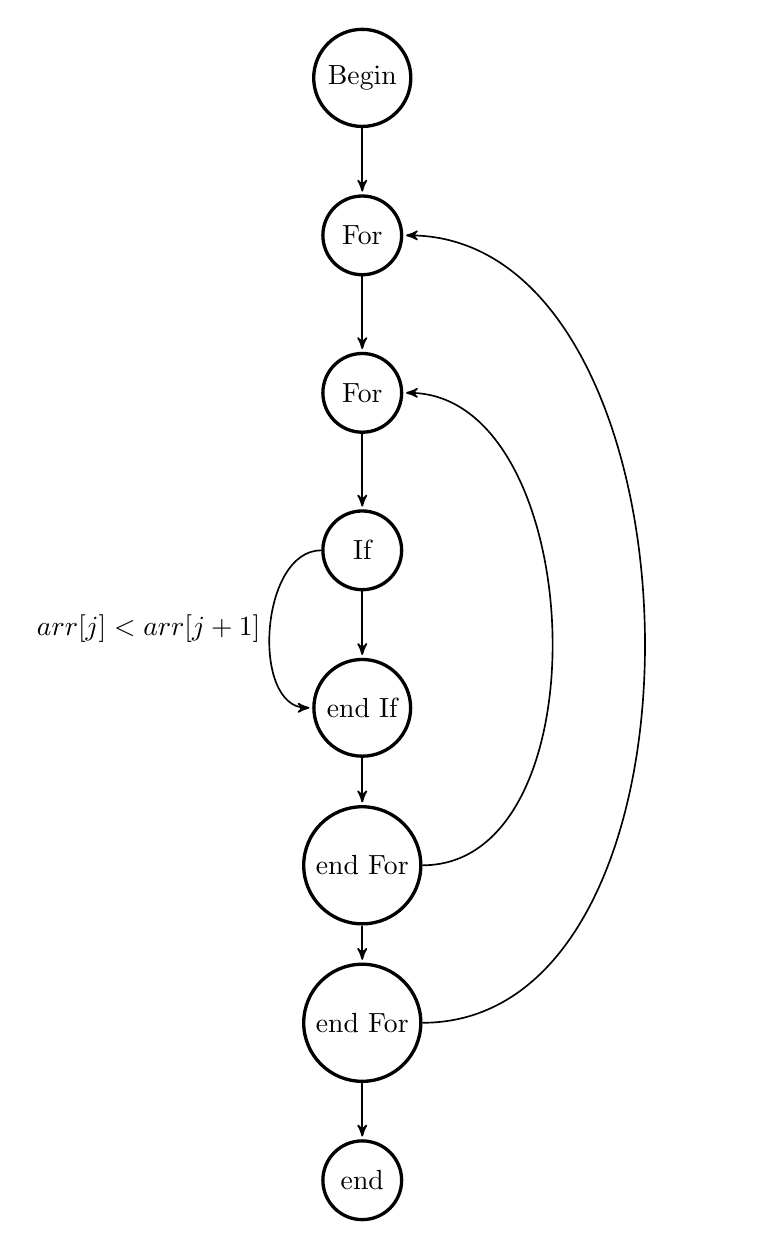
\begin{tikzpicture}[->, >=stealth', shorten >=1pt, auto, node distance=2cm, semithick,
roundnode/.style={circle, draw=black, very thick, minimum size=1cm}]
    \node[roundnode] (start) {Begin};
    \node[roundnode] [below of=start] (for1) {For};
    \node[roundnode] [below of=for1] (for2) {For};
    \node[roundnode] [below of=for2] (if) {If};
    \node[roundnode] [below of=if] (ifEnd) {end If};
    \node[roundnode] [below of=ifEnd] (forEnd2) {end For};
    \node[roundnode] [below of=forEnd2] (forEnd1) {end For};
    \node[roundnode] [below of=forEnd1] (end) {end};

    \path
      (start) edge (for1)
      (for1) edge (for2)
      (for2) edge (if)
      (if) edge (ifEnd)
           edge[left,in=-180,out=-180] node {$arr[j] < arr[j+1]$} (ifEnd)
      (ifEnd) edge (forEnd2)
      (forEnd2) edge (forEnd1)
      (forEnd1) edge (end)

      (forEnd2) edge[left,in=0,out=0] (for2)
      (forEnd1) edge[right,in=0,out=0] (for1);
  \end{tikzpicture}
\end{center}
\end{document}